\chapter{Question 2}
\label{avoiding-uri-aliases} 

\textbf{ We know the group split in two different groups.  Suppose the disagreements in the group were more nuanced -- what would the clubs look like if they split into groups of 3, 4, and 5?}

\begin{itemize}
\item I continued iterating till I get groups of 3, 4 and 5.
\newpage
\item I got the partitioned graph with 3 groups in 14th iteration. The resultant graph for each iteration with highlighted edges is illustrated in Figures \ref{fig:q2fig1}, \ref{fig:q2fig2}, \ref{fig:q2fig3} and the output graph with 3 groups is in Figure \ref{fig:q2fig4}.
\begin{figure}[h!]
\begin{center}
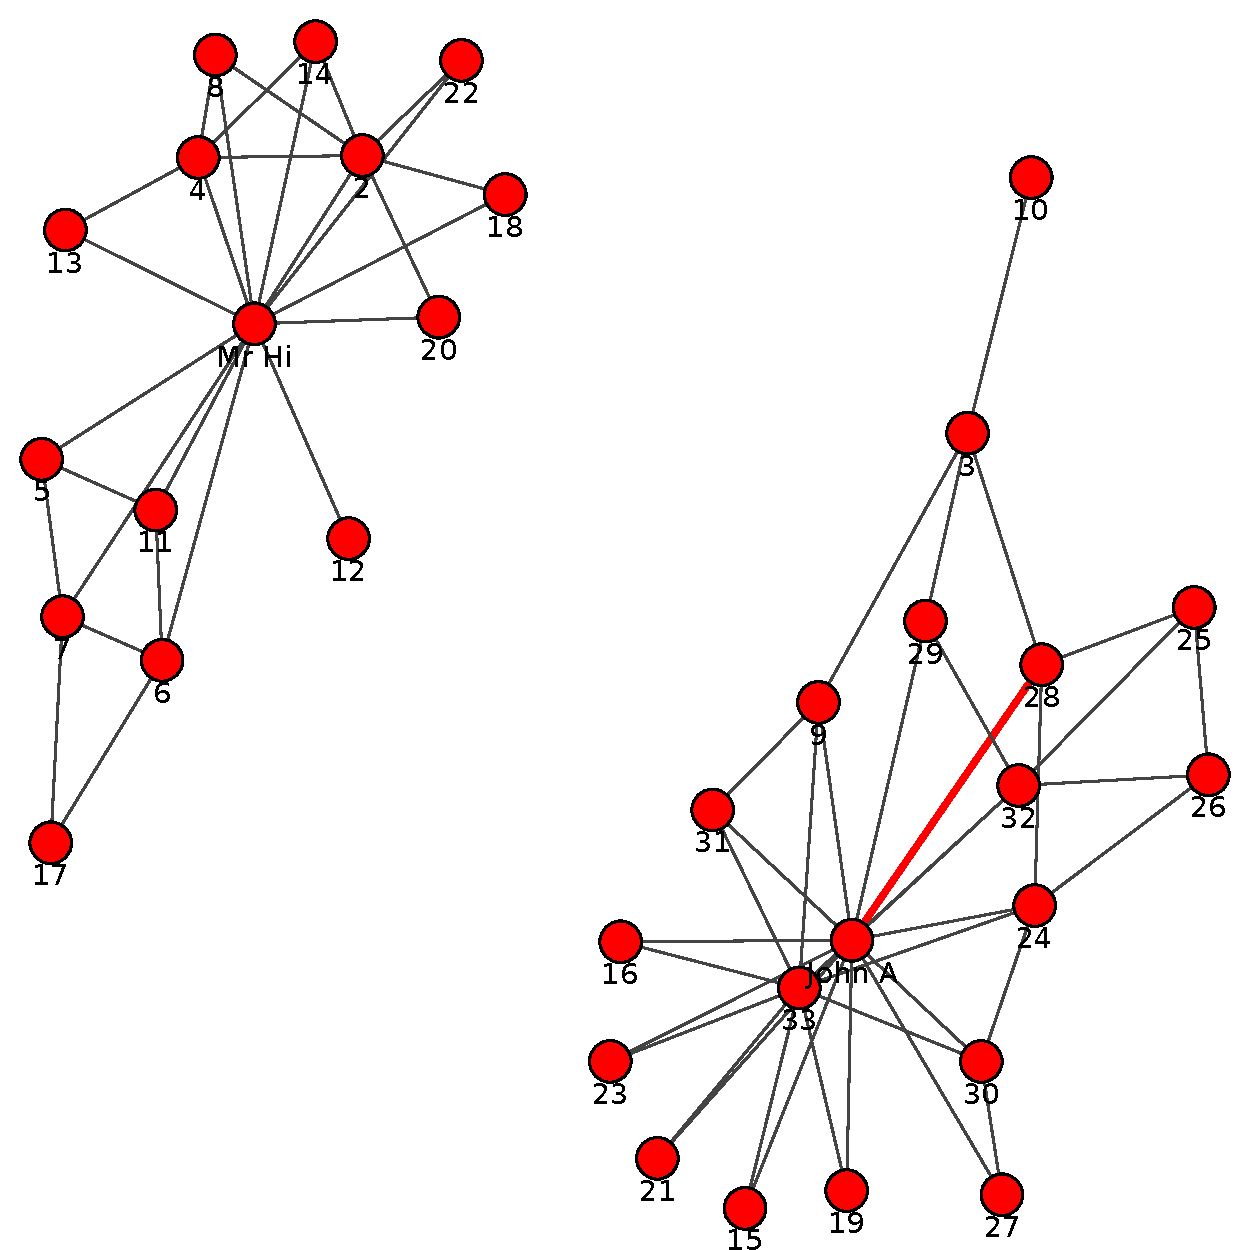
\includegraphics[scale=0.55, keepaspectratio=true]{figures/graphs/EdgeHighlightedGraph12.pdf}
\caption{Iteration 12}
\label{fig:q2fig1}
\end{center}
\end{figure}
\newpage
\begin{figure}[h!]
\begin{center}
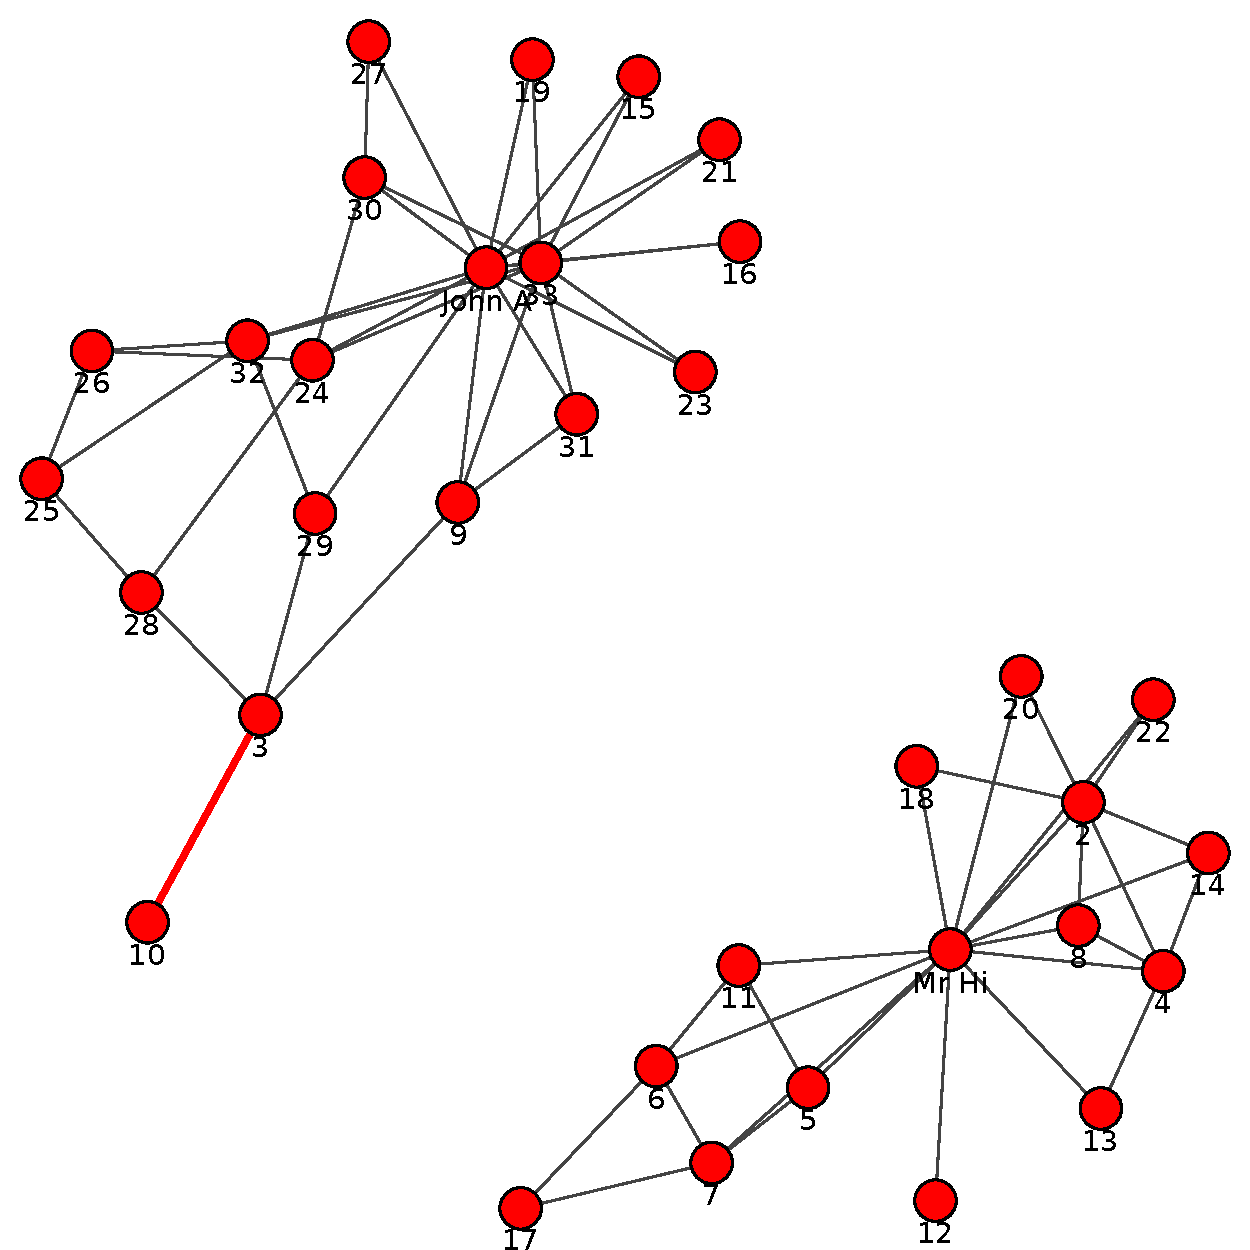
\includegraphics[scale=0.55, keepaspectratio=true]{figures/graphs/EdgeHighlightedGraph13.pdf}
\caption{Iteration 13}
\label{fig:q2fig2}
\end{center}
\end{figure}
\newpage
\begin{figure}[h!]
\begin{center}
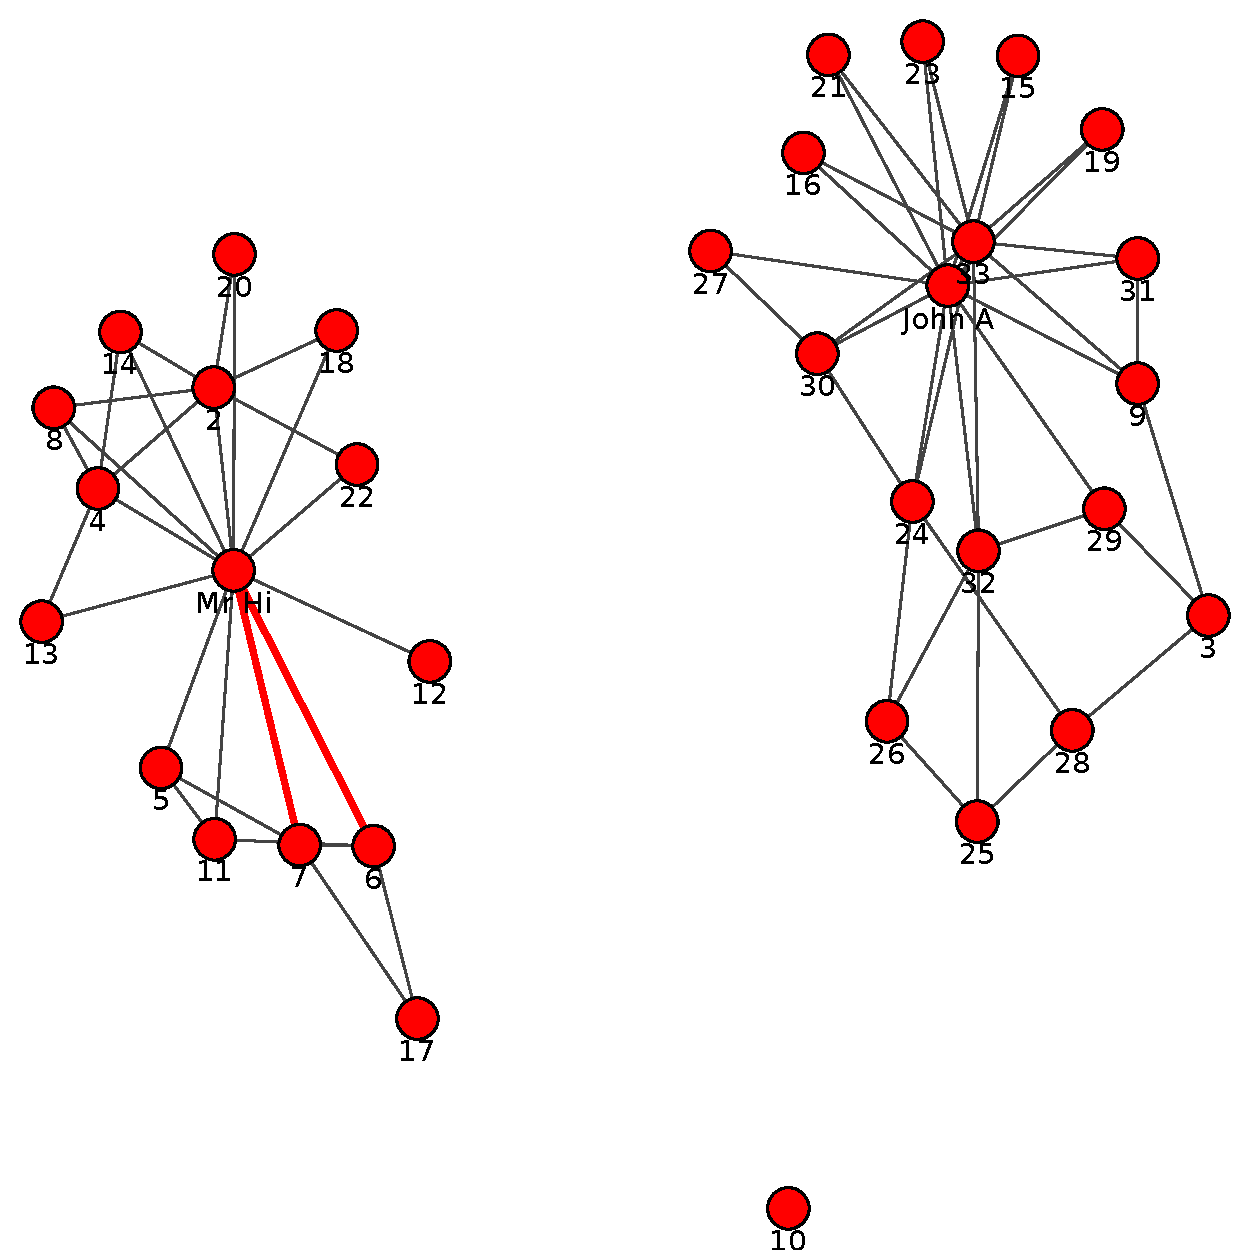
\includegraphics[scale=0.55, keepaspectratio=true]{figures/graphs/EdgeHighlightedGraph14.pdf}
\caption{Iteration 14}
\label{fig:q2fig3}
\end{center}
\end{figure}
\newpage
\begin{figure}[h!]
\begin{center}
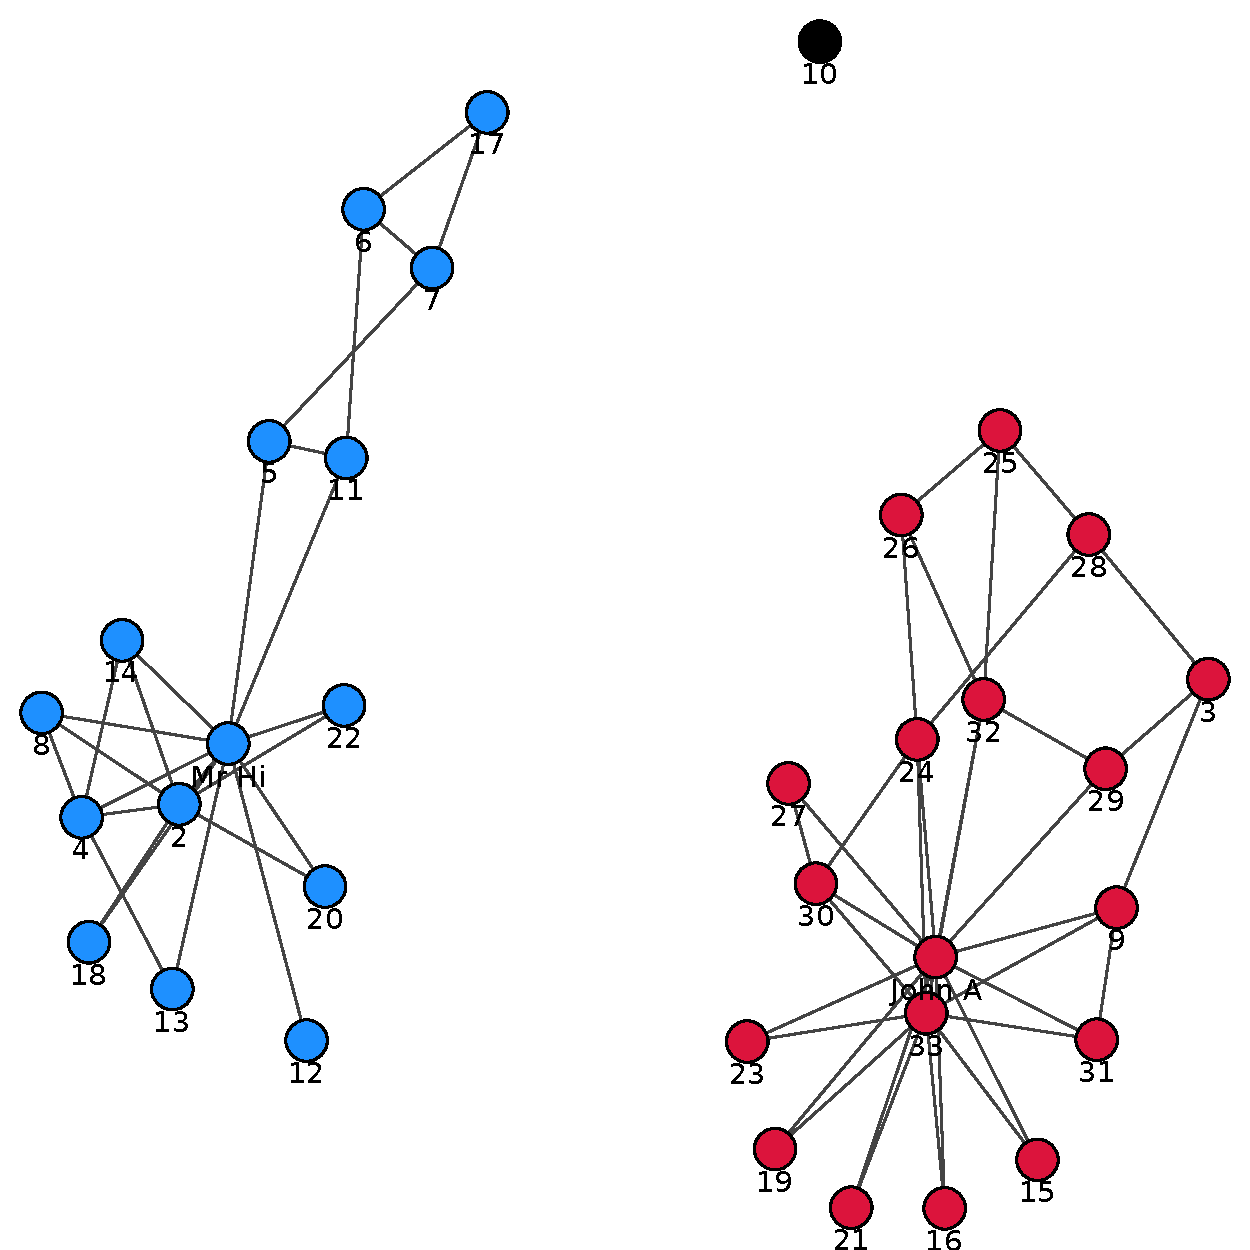
\includegraphics[scale=0.55, keepaspectratio=true]{figures/graphs/GraphWith3Groups.pdf}
\caption{Output of Girvan Newman algorithm which divides the Karate Club Graph divided into 3 groups}
\label{fig:q2fig4}
\end{center}
\end{figure}
\newpage
\item I got the partitioned graph with 4 groups in 16th iteration. The resultant graph for each iteration with highlighted edges is illustrated in Figures \ref{fig:q2fig1}, \ref{fig:q2fig2}, \ref{fig:q2fig3} and the output graph with 3 groups is in Figure \ref{fig:q2fig4}.
\begin{figure}[h!]
\begin{center}
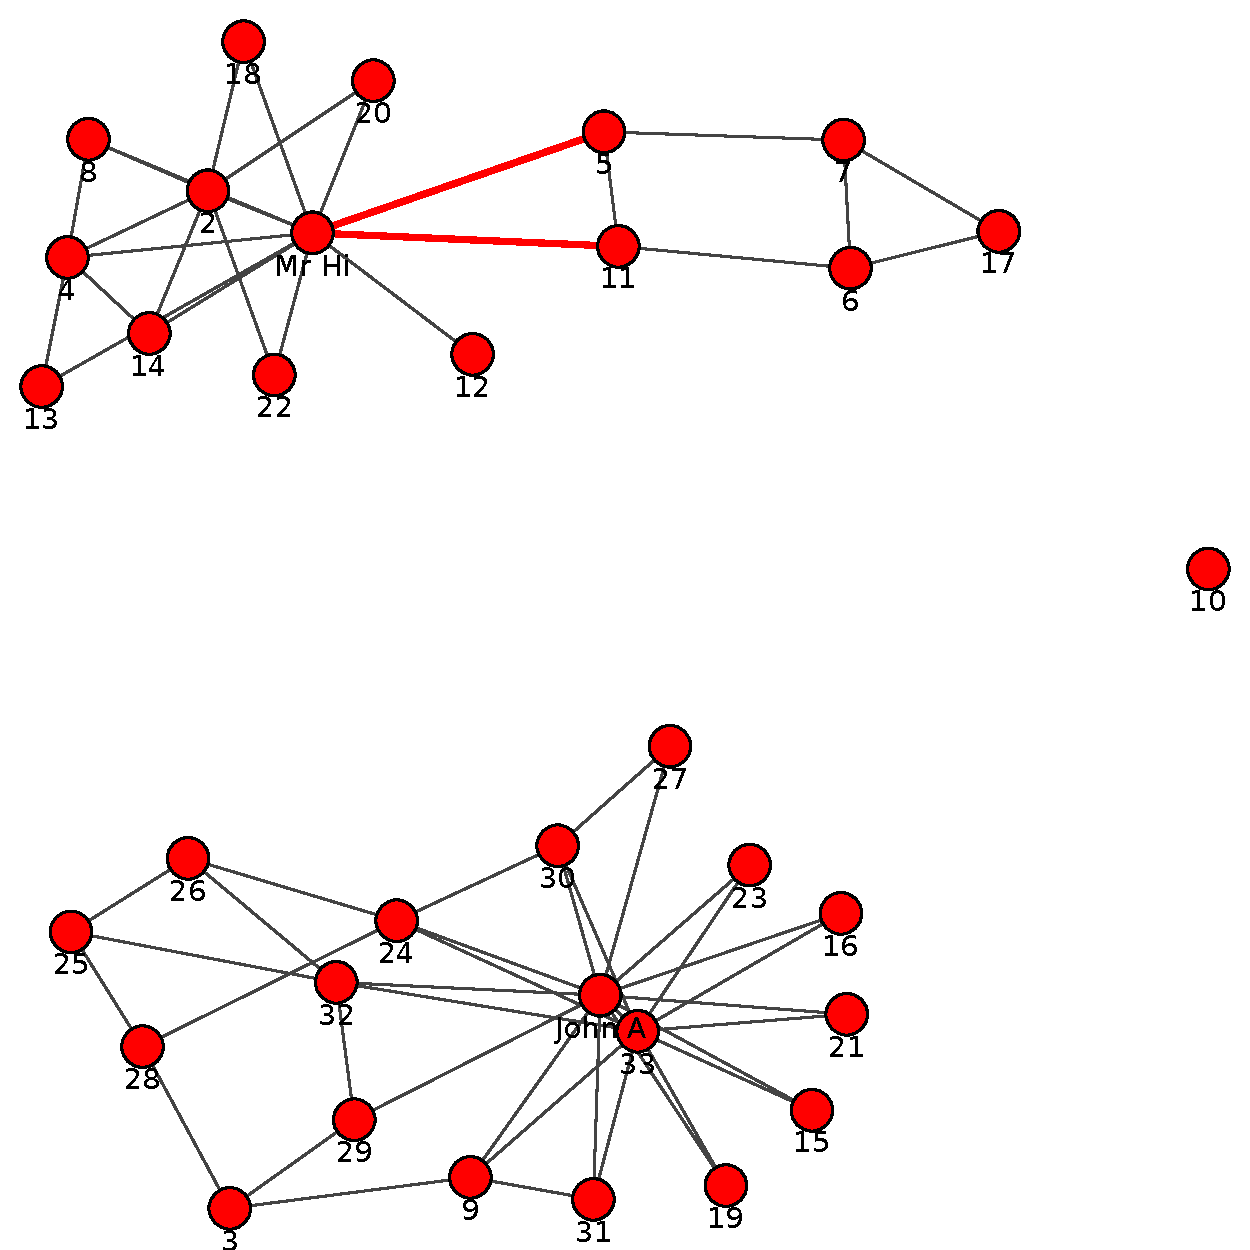
\includegraphics[scale=0.55, keepaspectratio=true]{figures/graphs/EdgeHighlightedGraph15.pdf}
\caption{Iteration 15}
\label{fig:q2fig5}
\end{center}
\end{figure}
\newpage
\begin{figure}[h!]
\begin{center}
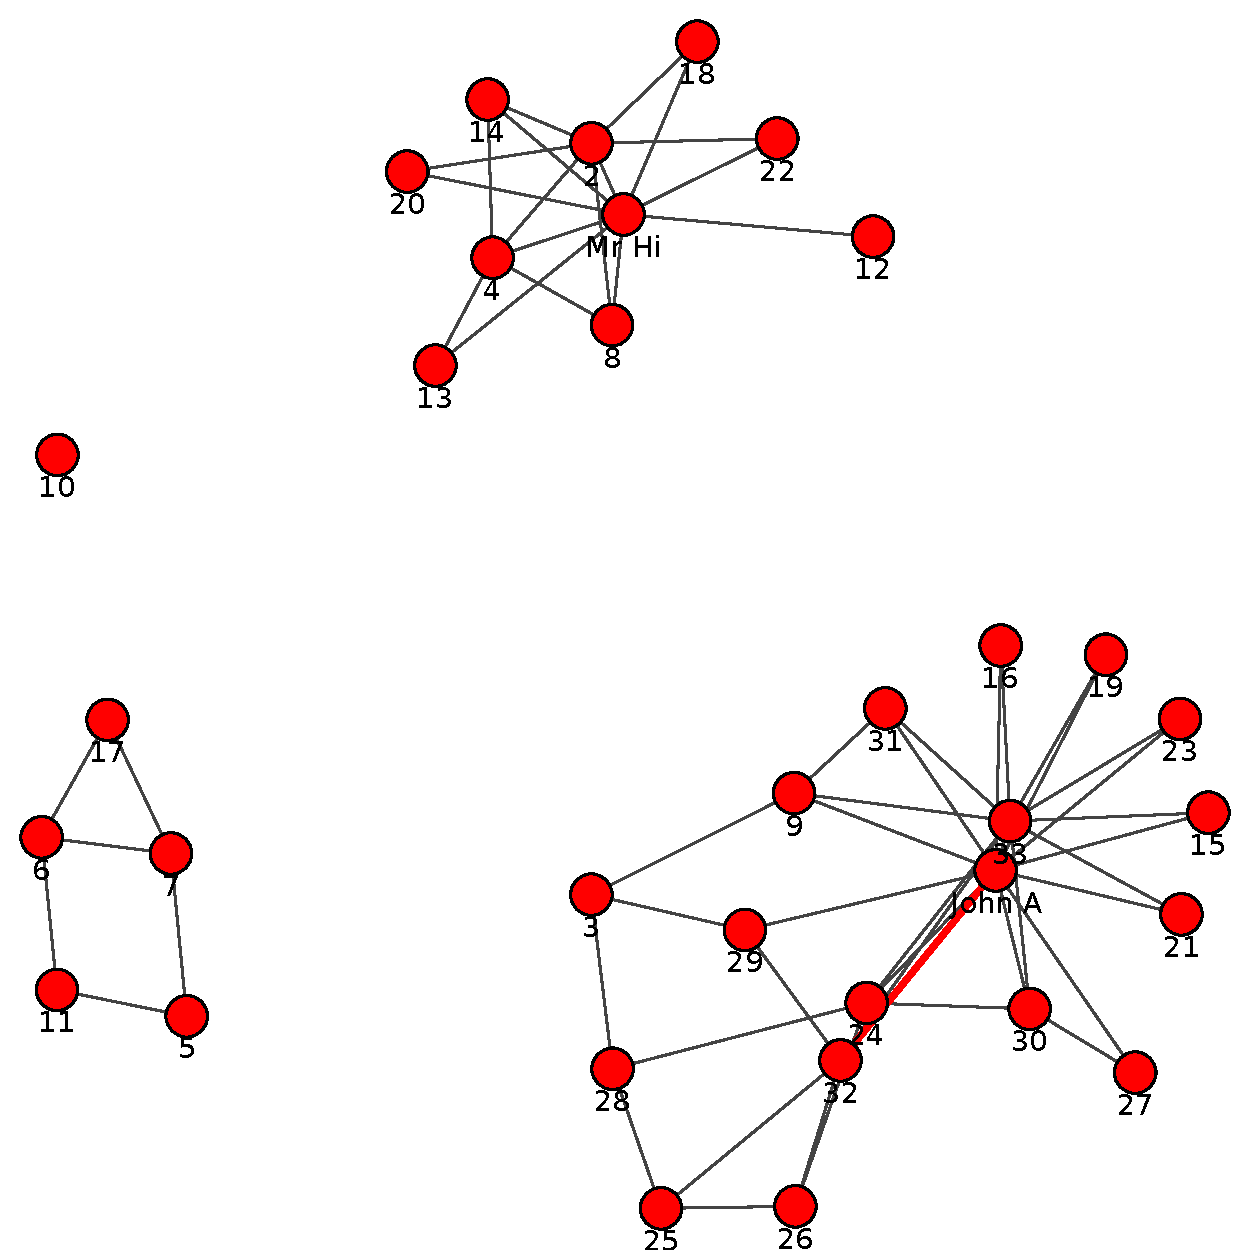
\includegraphics[scale=0.55, keepaspectratio=true]{figures/graphs/EdgeHighlightedGraph16.pdf}
\caption{Iteration 16}
\label{fig:q2fig6}
\end{center}
\end{figure}
\newpage
\begin{figure}[h!]
\begin{center}
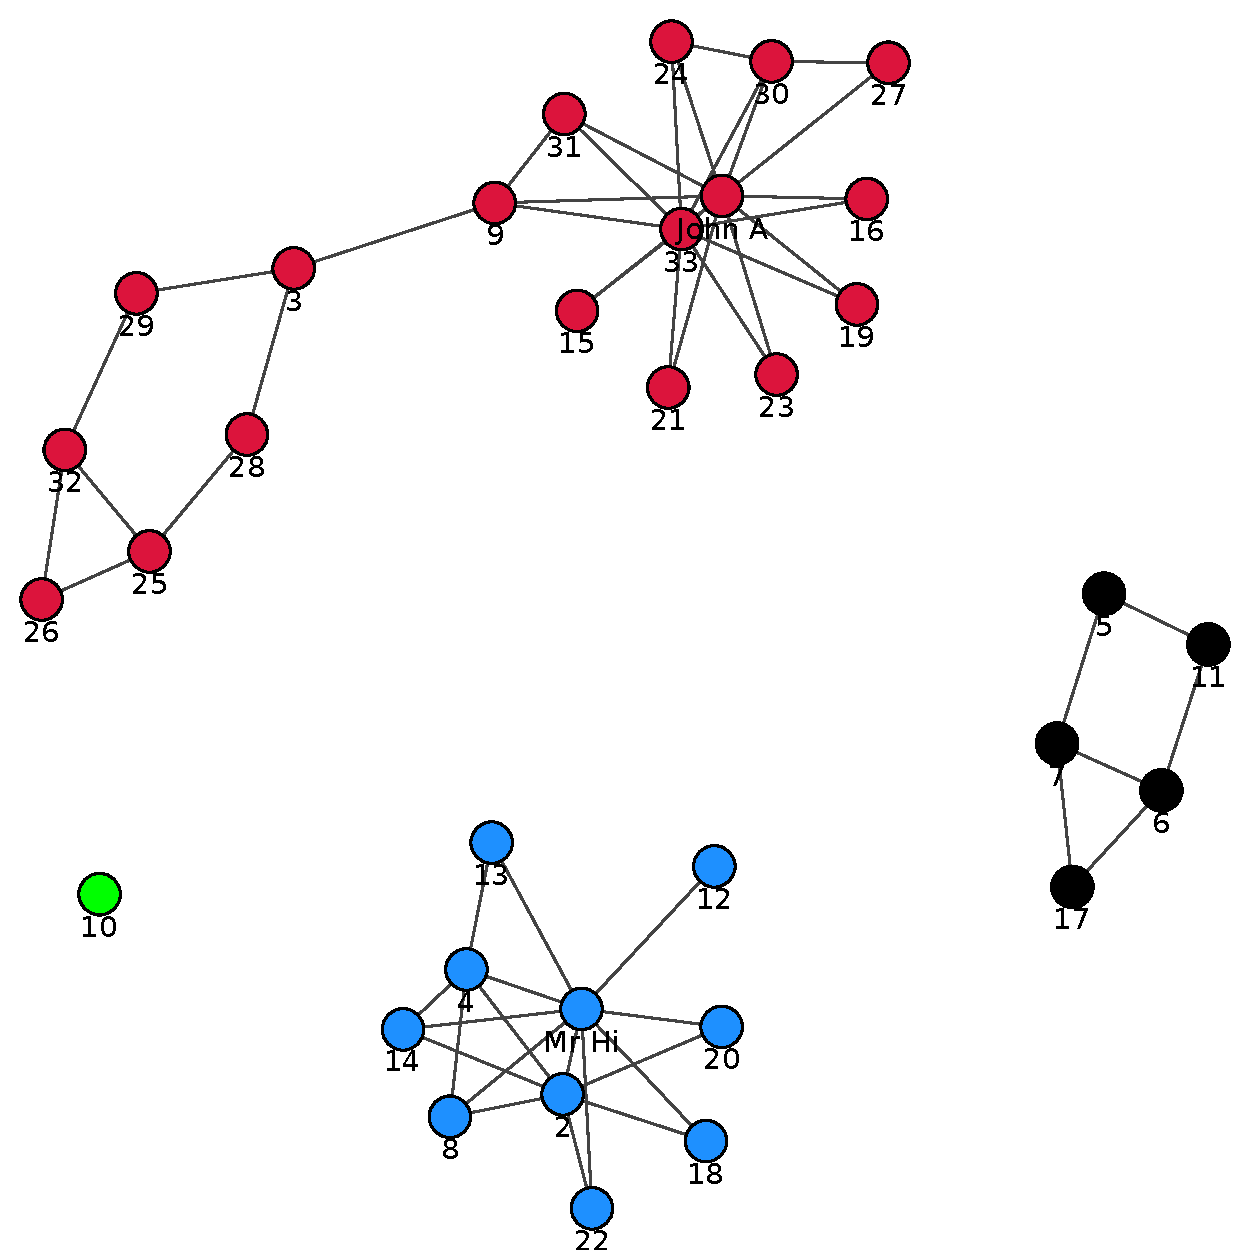
\includegraphics[scale=0.55, keepaspectratio=true]{figures/graphs/GraphWith4Groups.pdf}
\caption{Output of Girvan Newman algorithm which divides the Karate Club Graph divided into 4 groups}
\label{fig:q2fig7}
\end{center}
\end{figure}
\newpage
\item I got the partitioned graph with 3 groups in 21st iteration. The resultant graph for each iteration with highlighted edges is illustrated in Figures \ref{fig:q2fig1}, \ref{fig:q2fig2}, \ref{fig:q2fig3} and the output graph with 3 groups is in Figure \ref{fig:q2fig4}.
\begin{figure}[h!]
\begin{center}
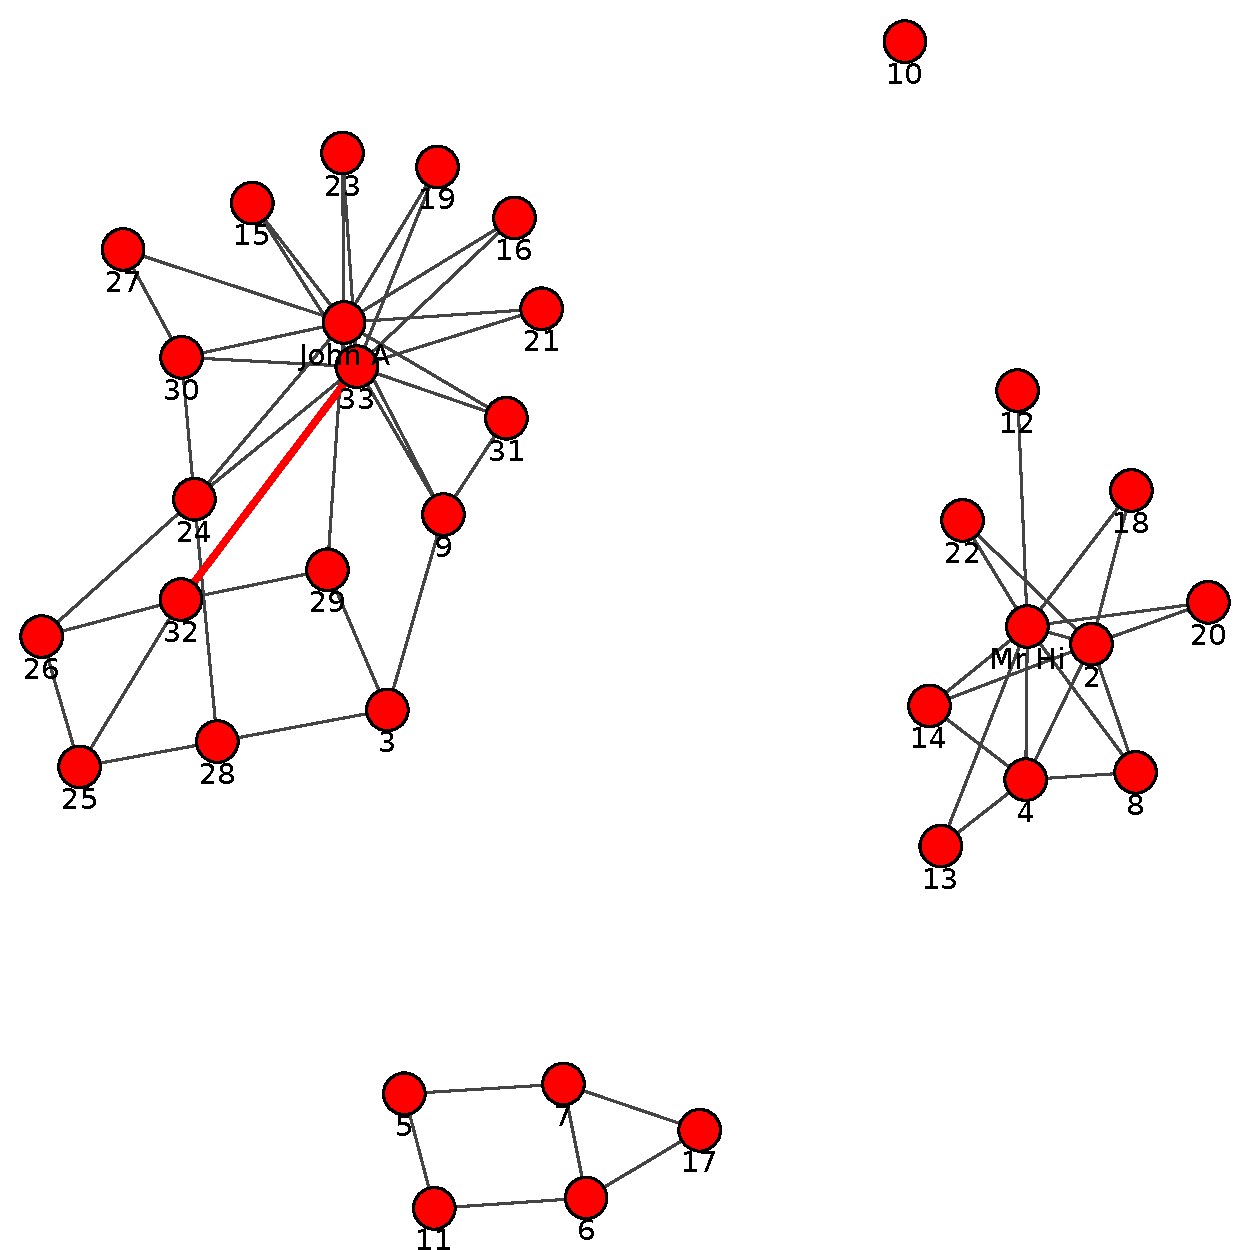
\includegraphics[scale=0.55, keepaspectratio=true]{figures/graphs/EdgeHighlightedGraph17.pdf}
\caption{Iteration 17}
\label{fig:q2fig8}
\end{center}
\end{figure}
\newpage
\begin{figure}[h!]
\begin{center}
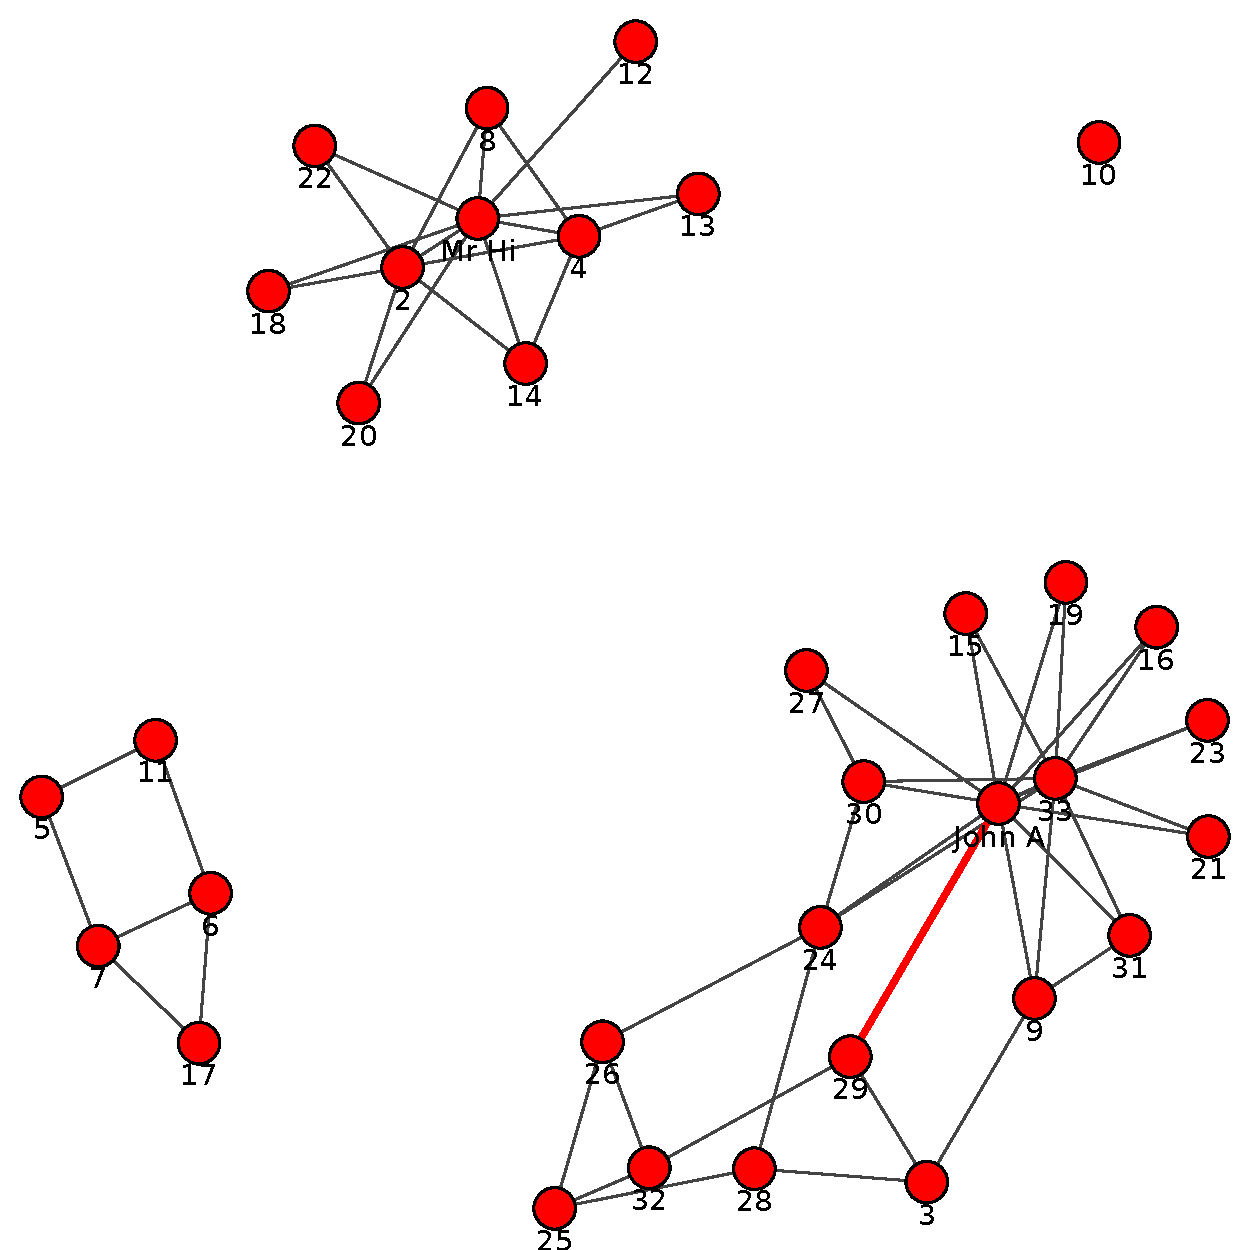
\includegraphics[scale=0.55, keepaspectratio=true]{figures/graphs/EdgeHighlightedGraph18.pdf}
\caption{Iteration 18}
\label{fig:q2fig9}
\end{center}
\end{figure}
\newpage
\begin{figure}[h!]
\begin{center}
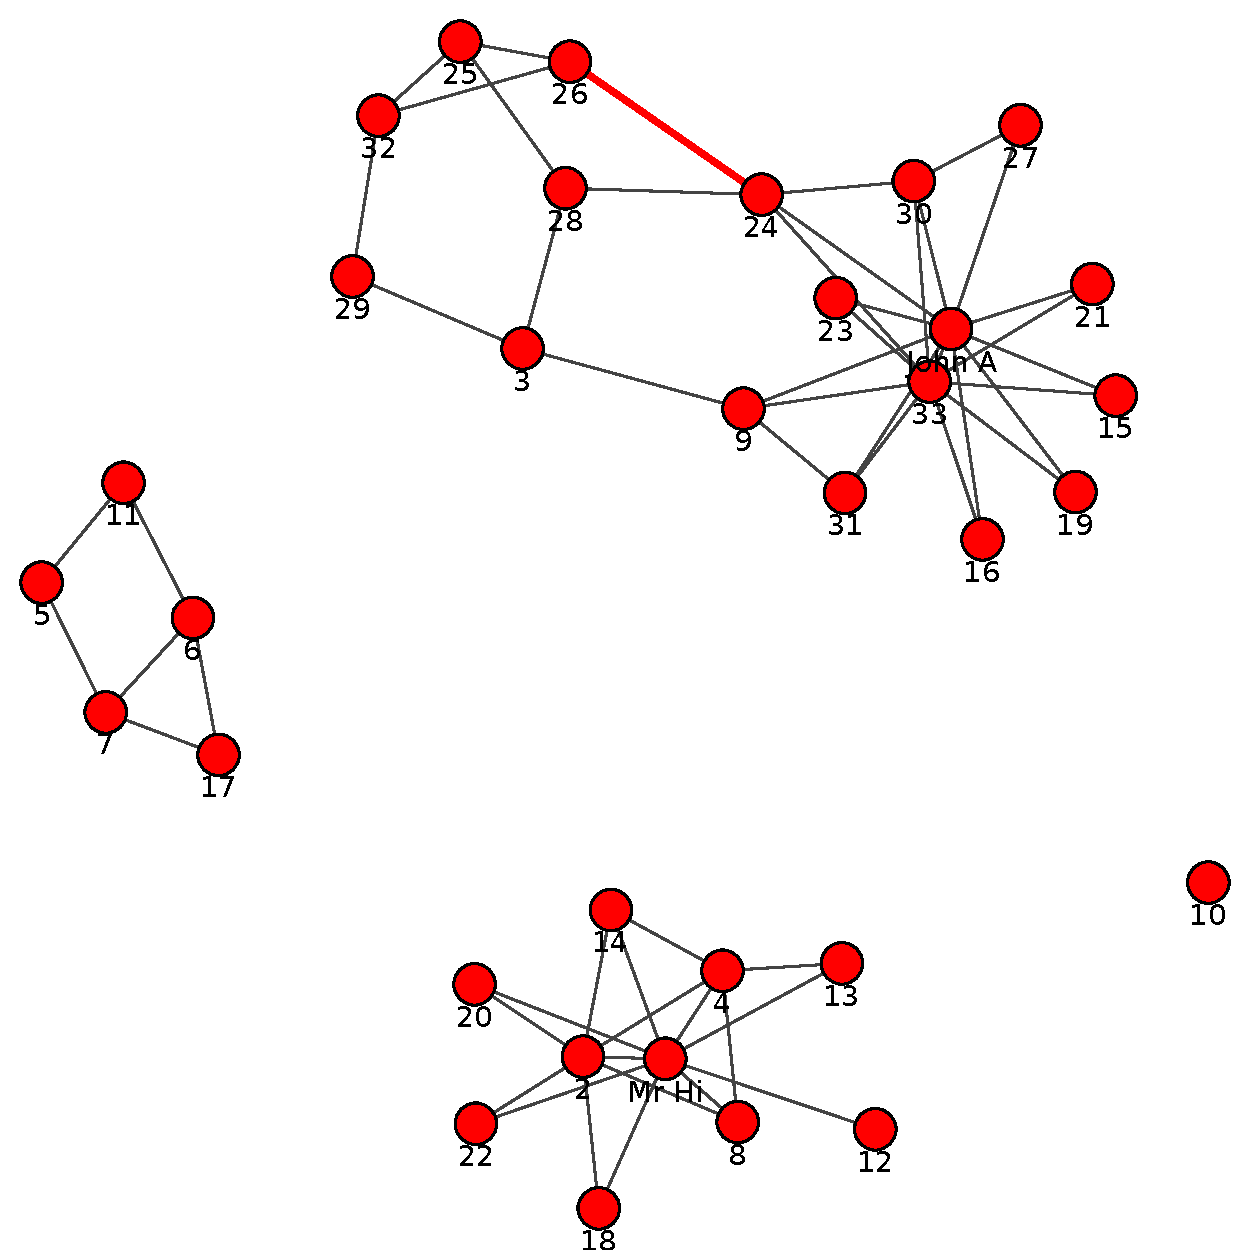
\includegraphics[scale=0.55, keepaspectratio=true]{figures/graphs/EdgeHighlightedGraph19.pdf}
\caption{Iteration 19}
\label{fig:q2fig10}
\end{center}
\end{figure}
\newpage
\begin{figure}[h!]
\begin{center}
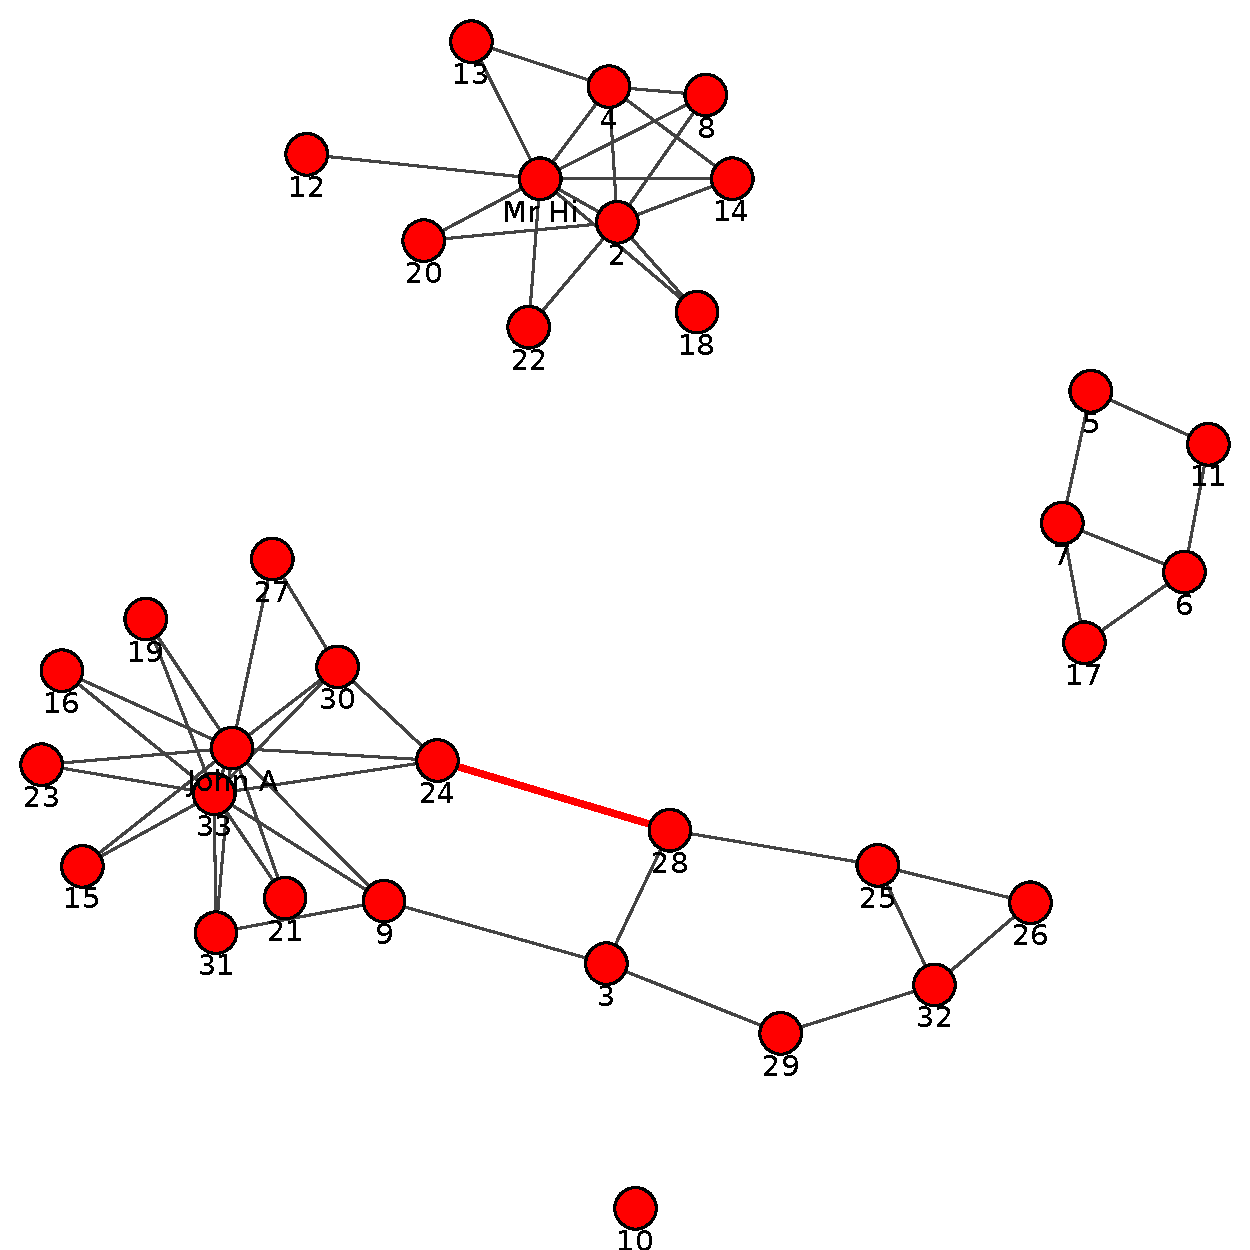
\includegraphics[scale=0.55, keepaspectratio=true]{figures/graphs/EdgeHighlightedGraph20.pdf}
\caption{Iteration 20}
\label{fig:q2fig11}
\end{center}
\end{figure}
\newpage
\begin{figure}[h!]
\begin{center}
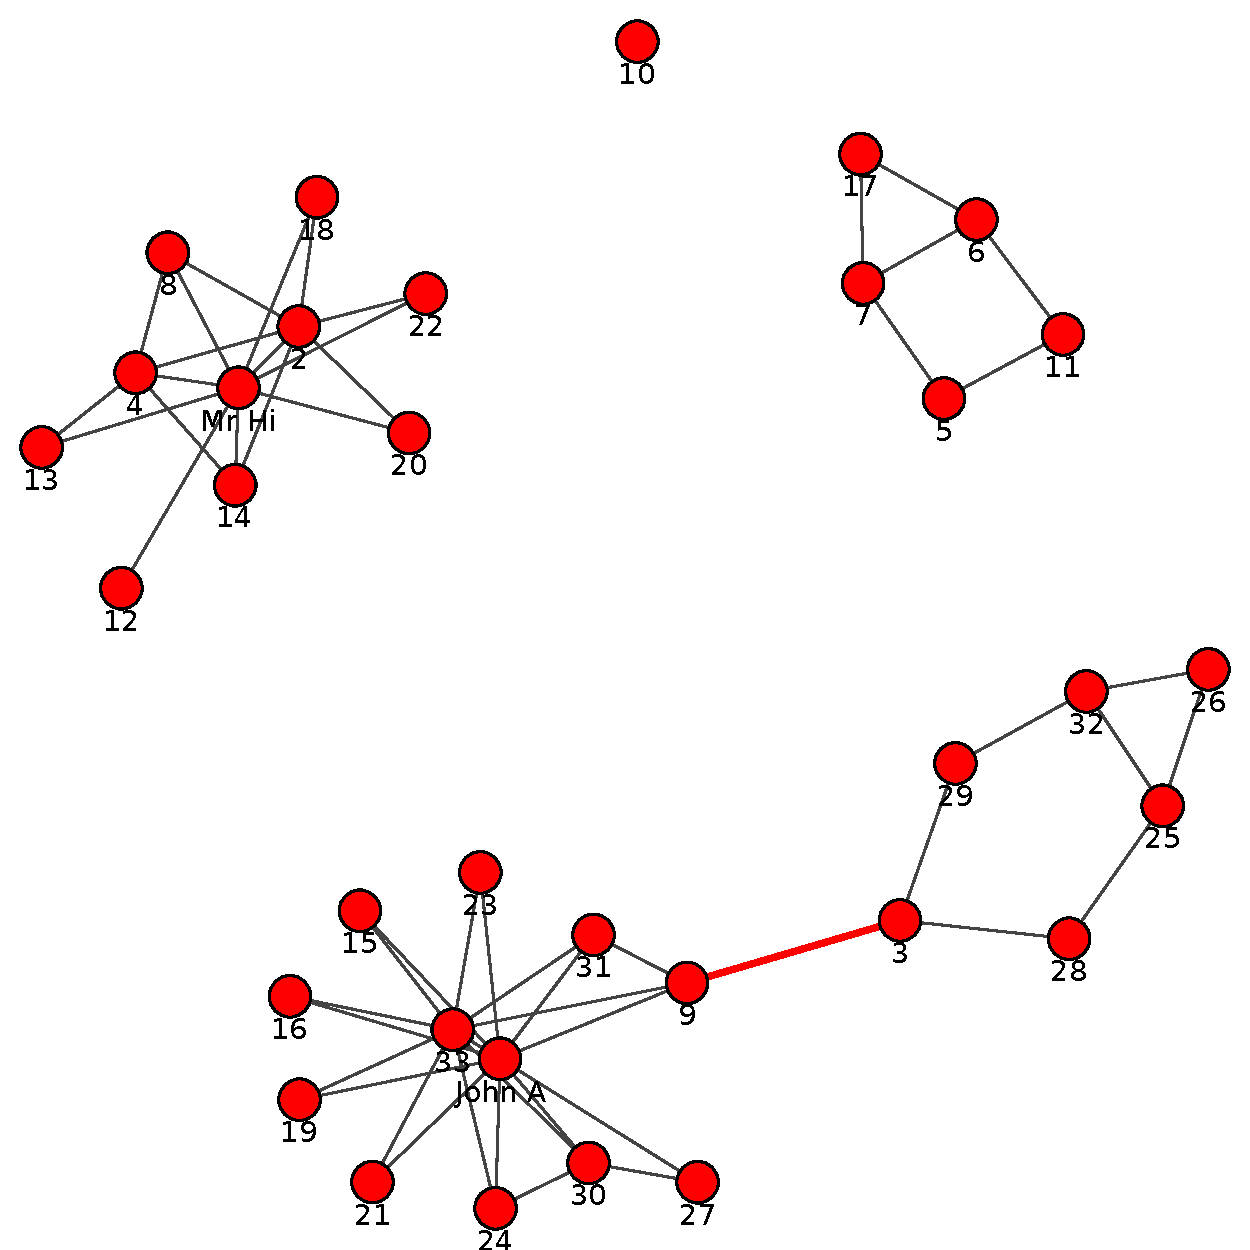
\includegraphics[scale=0.55, keepaspectratio=true]{figures/graphs/EdgeHighlightedGraph21.pdf}
\caption{Iteration 21}
\label{fig:q2fig12}
\end{center}
\end{figure}
\newpage
\begin{figure}[h!]
\begin{center}
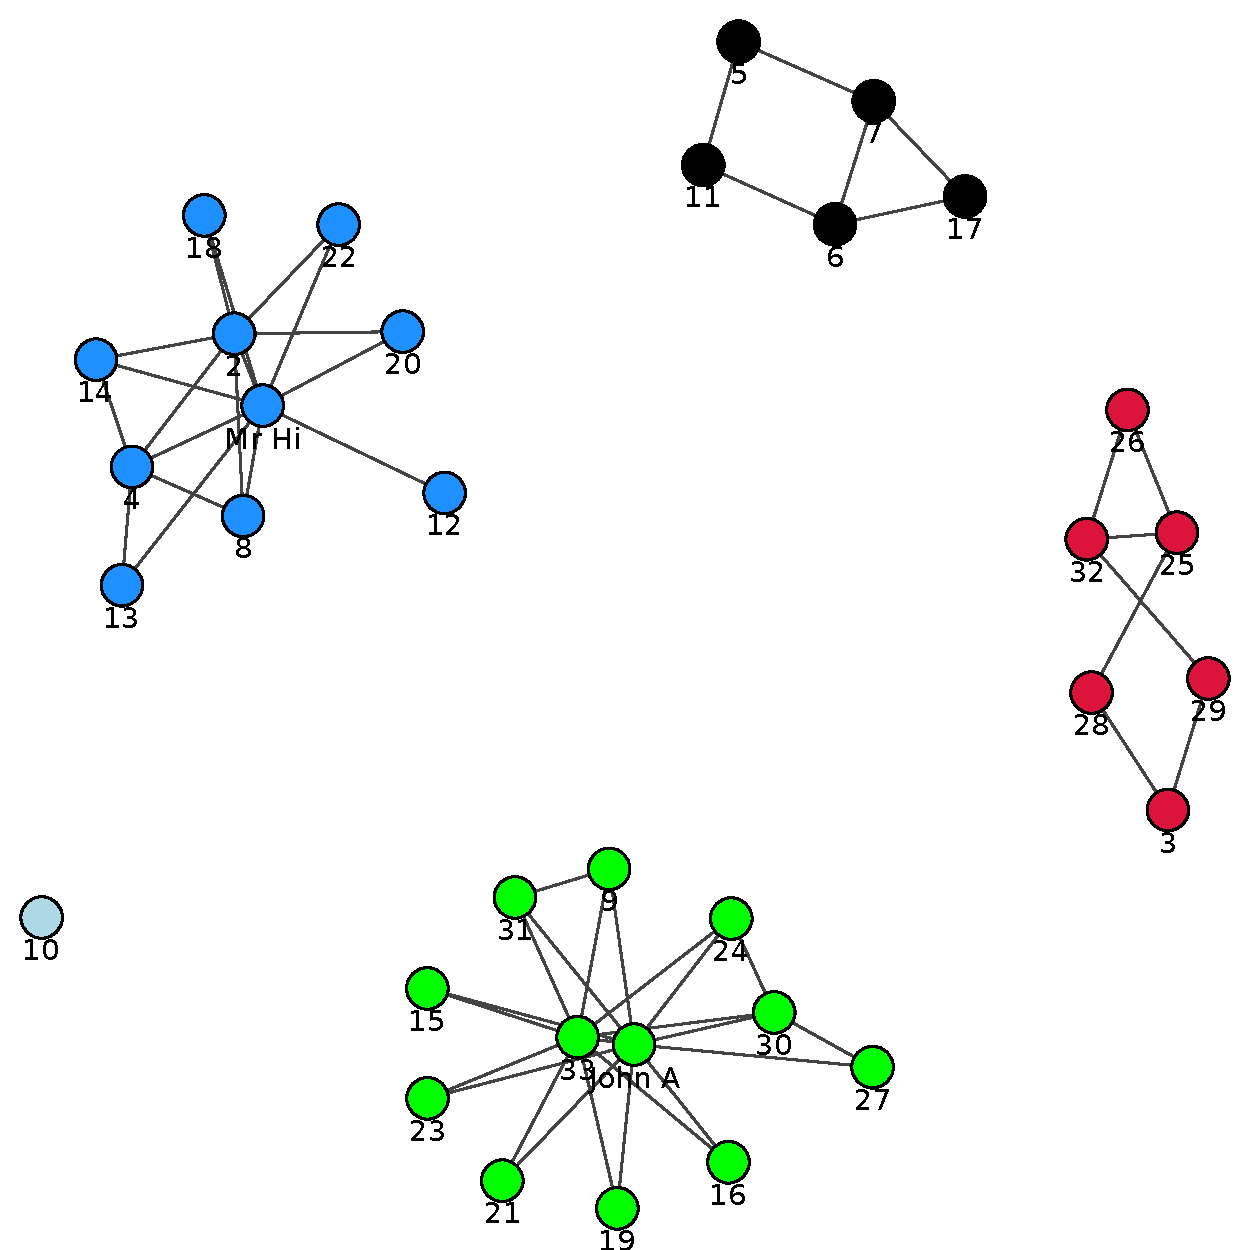
\includegraphics[scale=0.55, keepaspectratio=true]{figures/graphs/GraphWith5Groups.pdf}
\caption{Output of Girvan Newman algorithm which divides the Karate Club Graph divided into 5 groups}
\label{fig:q2fig13}
\end{center}
\end{figure}
\end{itemize}